%autobuild=true changelog

\documentclass[a4paper,9pt,DIV10,oneside,openany]{scrbook}
\usepackage{index}
\usepackage[onehalfspacing]{setspace}
\usepackage{bibgerm}
\usepackage{tabularx}
\usepackage{bibentry}
\usepackage{ifthen}

% new index for config registry variables
\makeindex
\newindex{ucsConfigRegistry}{ndx}{nnd}{Univention Config Registry-Variablen}

% mini table of contents, we have to redefine text styles used
\usepackage[germanb]{minitoc-hyper}
\def\mtcfont{\small\sf}
\def\mtcSfont{\small\sf}
\def\mtifont{\large\sf}

% new command for chapters
\newcommand{\ucsChapter}[1]{\chapter{#1} \minitoc}

% packages needed in all documents

\usepackage[T1]{fontenc}
\usepackage[utf8]{inputenc}
\usepackage{ngerman}
\usepackage{verbatim}
\usepackage[hyphens,spaces]{url}
\usepackage{listings}
\usepackage{lastpage}
\usepackage{graphicx}
\usepackage{ifthen}
\usepackage{index}
\usepackage{color}
\usepackage{placeins}
\usepackage{float}
\usepackage{longtable}
\usepackage{pifont}
\usepackage{version}
\usepackage{multirow}
\usepackage{eso-pic}
\usepackage{wallpaper}
\usepackage[top=4.5cm, headsep=1.5cm, bottom=3cm, footskip=2cm]{geometry}
%\usepackage{showkeys}  % ENABLE SHOWKEYS TO DISPLAY REFERENCE_TAGS IN DOCUMENT
\usepackage{ucsframed}
\usepackage{marginnote}
\usepackage{placeins}

\def\UrlBreaks{\do\/\do\.\do\-}

\iftrue
% http://www.ctan.org/tex-archive/macros/latex/required/psnfss/psnfss2e.pdf
\usepackage{mathptmx} % roman, formulas
\usepackage{helvet} % sans-serif
\usepackage{courier} % typewriter
\renewcommand{\familydefault}{\sfdefault}
\else
% use font univers as sf-font
\fontfamily{pun}
\selectfont
\sffamily
\renewcommand*{\rmdefault}{pun} % pageheader
\renewcommand*{\sfdefault}{pun} % global font
%\renewcommand*{\ttdefault}{pun} % fixed font, should not be univers
\fi

% Tabbox, can be used to create s.th. like this
%
% ---------------------
% | Tab-Titel         |
% ------------------------------------
% | whatever you want                |
% | and some more of this            |
% ------------------------------------
%
% usage:
%
% \begin{ucsTabbox}{Tab-Titel}
% whatever you want
% and some more of this
% \end{ucsTabbox}

% Tabbox with Info Sign

\newenvironment{ucsInfobox}[1]
{\marginpar{\vspace{3ex}\centering
\includegraphics{abbildungen/info.jpg}}\setlength{\FrameRule}{1pt}\setlength{\fboxsep}{2mm}\begin{ucsframed}{#1}\parskip\baselineskip}
{\end{ucsframed}}

\newenvironment{ucsTabbox}[1]
{\setlength{\FrameRule}{1pt}\setlength{\fboxsep}{2mm}\begin{ucsframed}{#1}\parskip\baselineskip}
{\end{ucsframed}}

\newcommand{\ucsTabentry}[2]{\textbf{#1}\\#2}

%% for the background-image on the title page
%% http://stackoverflow.com/questions/240097/how-to-create-a-background-image-on-titlepage-with-latex
\newcommand\BackgroundPicEven{
\put(0,0){
\parbox[b][\paperheight]{\paperwidth}{%
\vfill
\centering
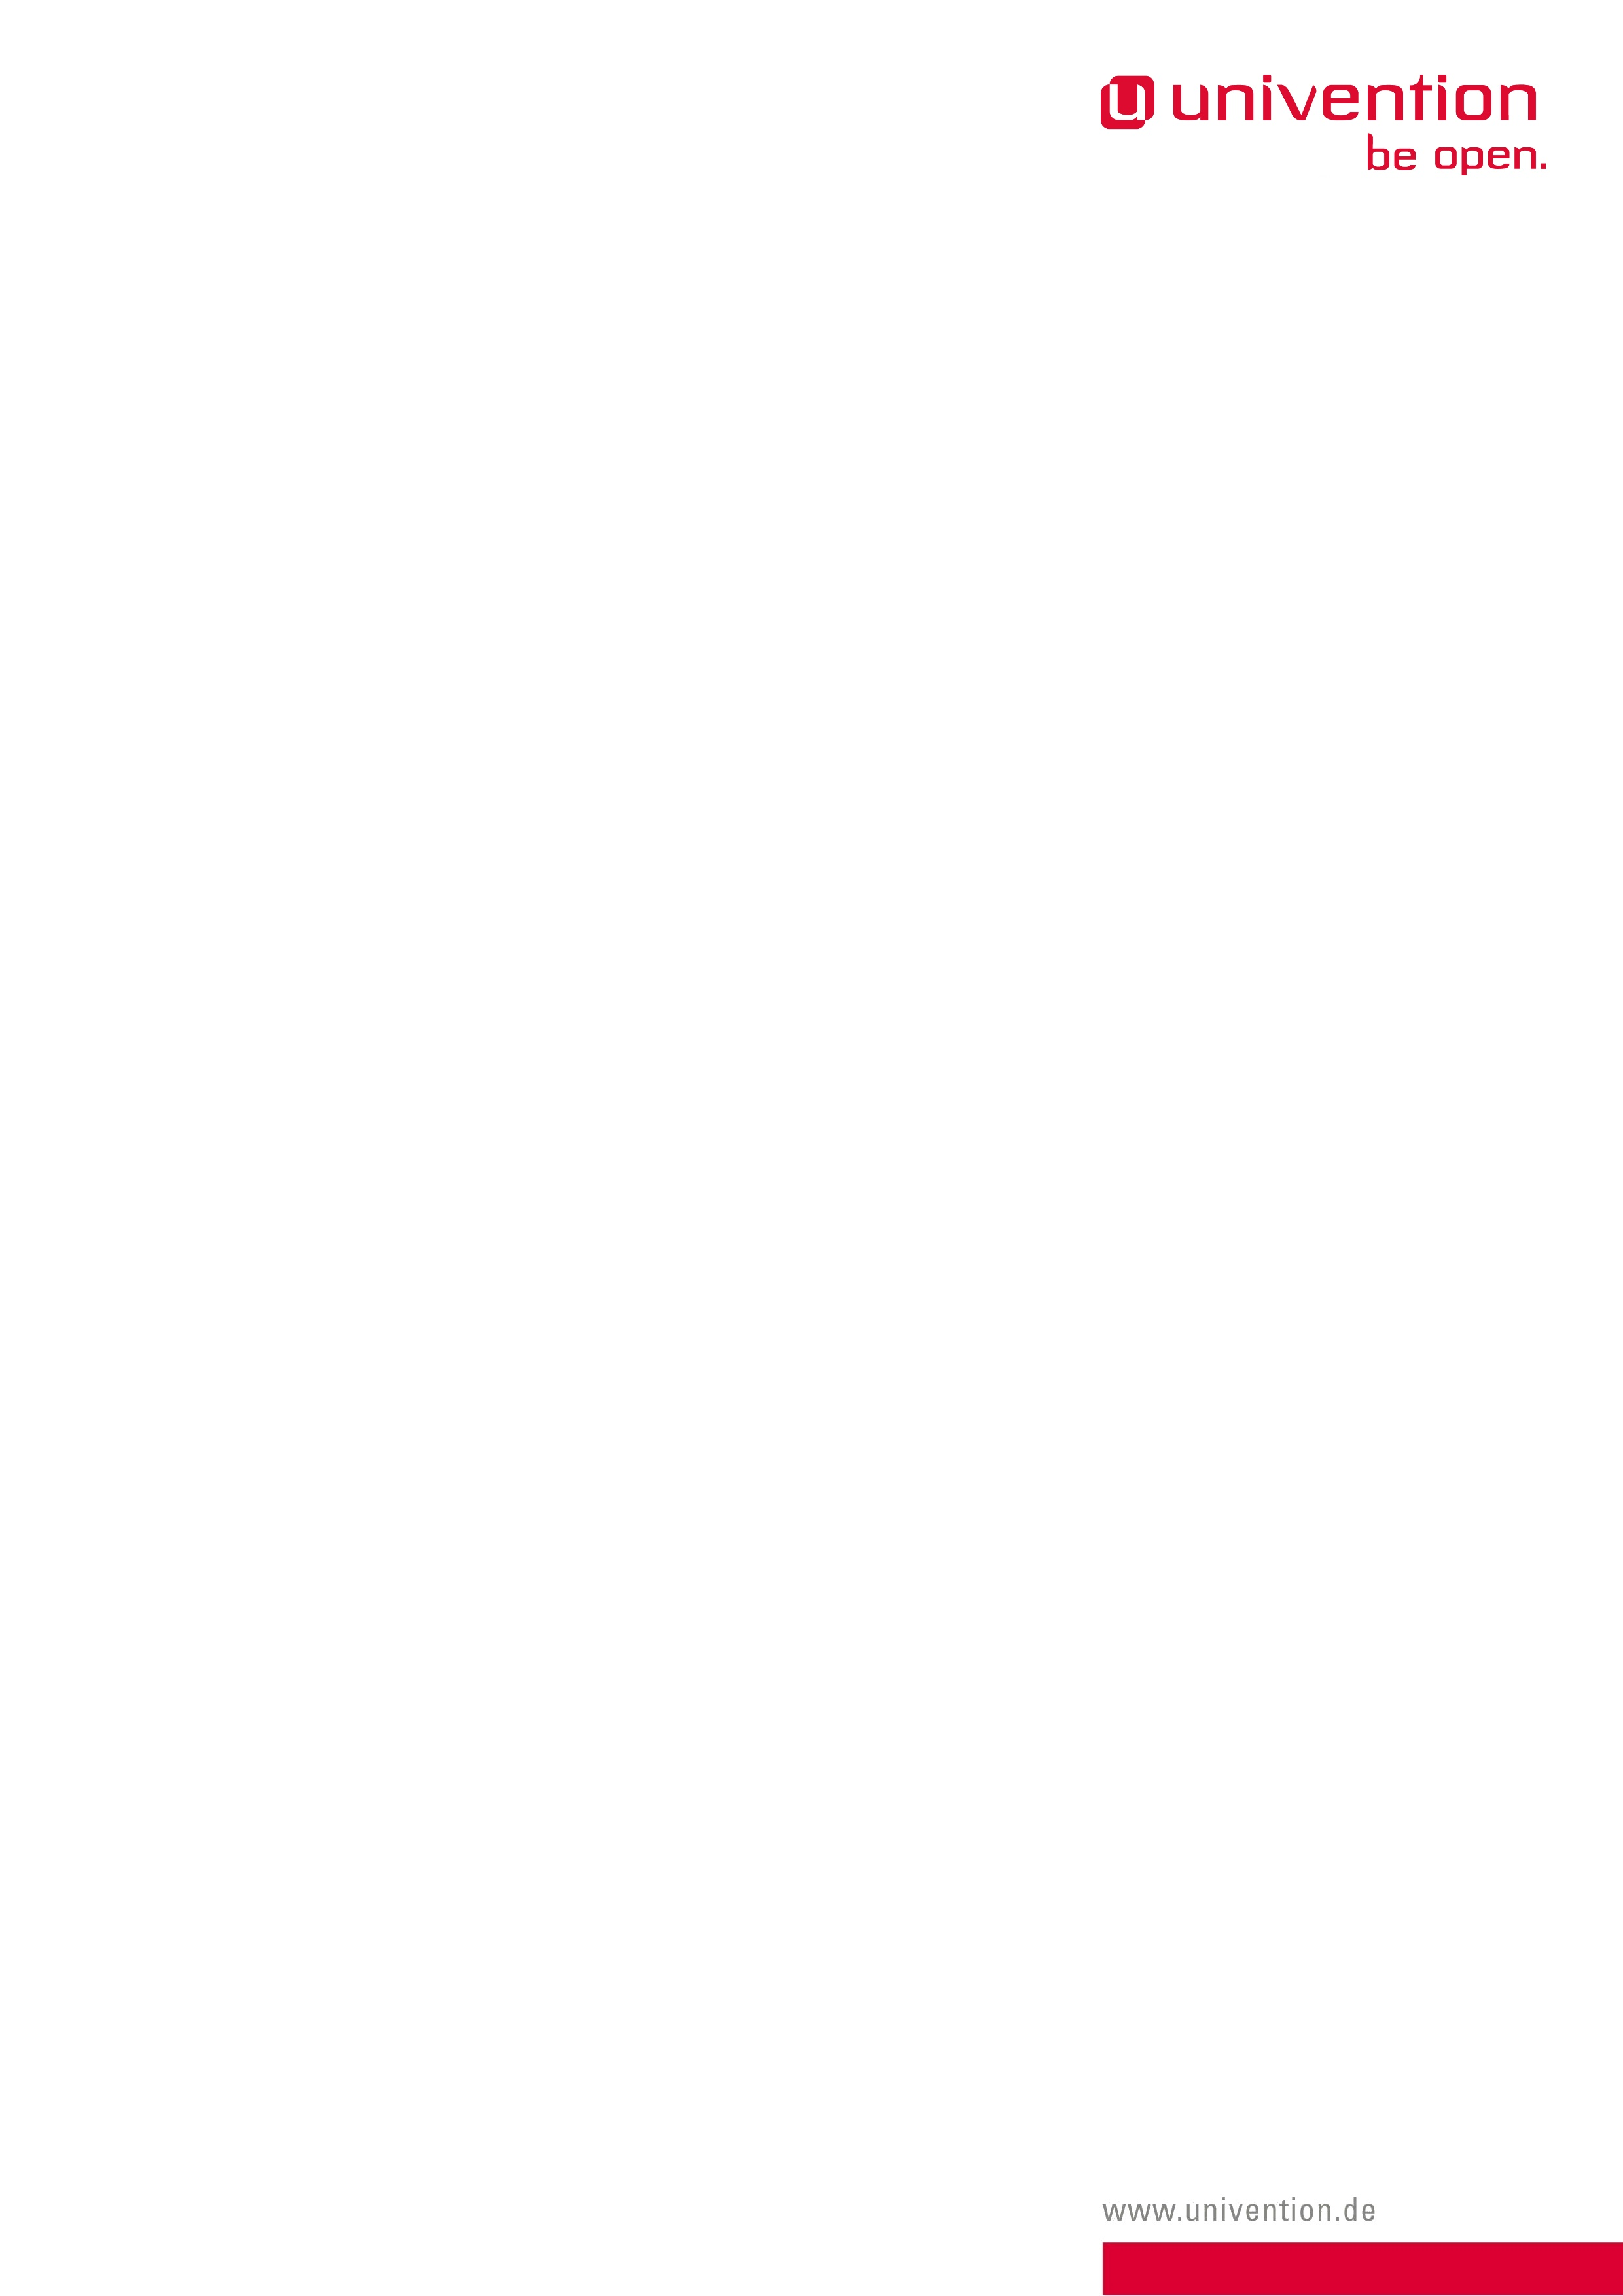
\includegraphics[width=\paperwidth,height=\paperheight]{illustrations/page-background-even.jpg}%
\vfill
}}}

\newcommand\BackgroundPicOdd{
\put(0,0){
\parbox[b][\paperheight]{\paperwidth}{%
\vfill
\centering
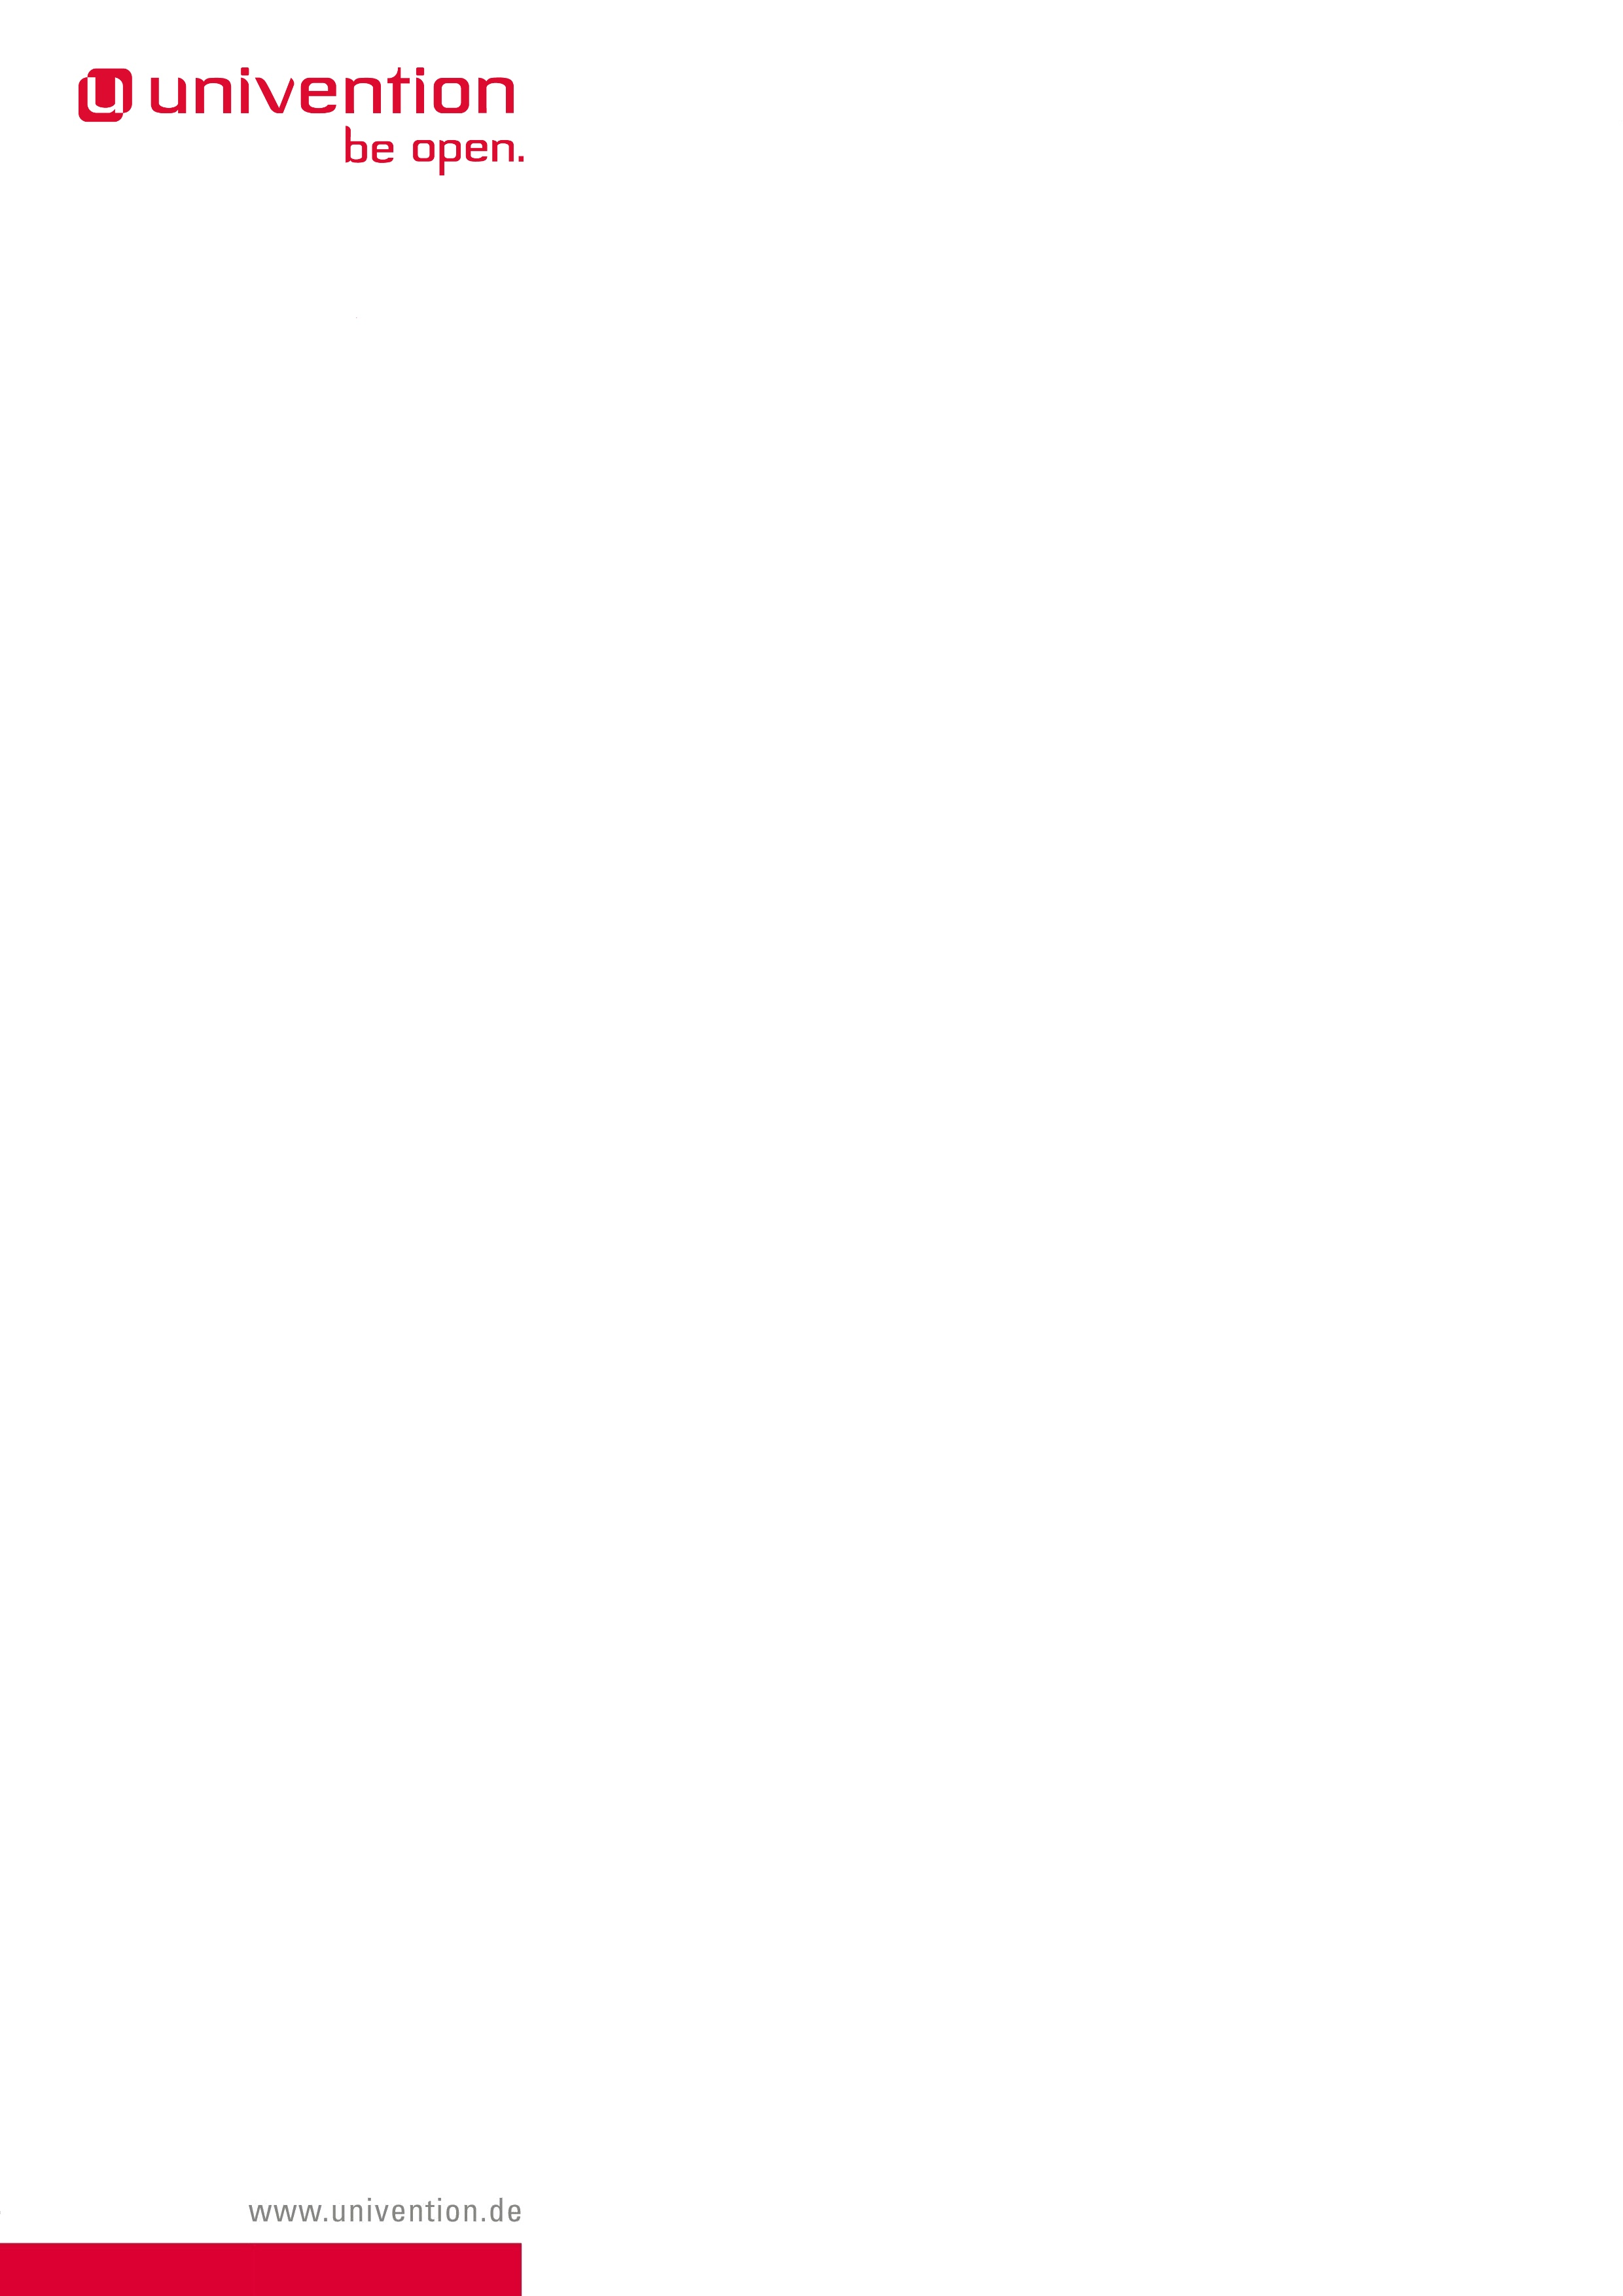
\includegraphics[width=\paperwidth,height=\paperheight]{illustrations/page-background-odd.jpg}%
\vfill
}}}

% Colors:
% red as used in univention corporate identiy
% gray for listing background

\definecolor{ucsRed}{RGB}{0.51372549, 0.141176471, 0.235294118}
\definecolor{ucsCodeGray}{gray}{0.7}
\definecolor{ucsHyperrefLinkColor}{rgb}{0, 0, 0.8}

% tabular environment using sans serif

\newenvironment{tableSansSerif}%
{\begin{table}[H]\footnotesize\sffamily}%
{\end{table}}

% environment for console sessions
\lstnewenvironment{ucsConsoleInput}
 {\lstset{basicstyle=\ttfamily}\small}
 {\normalsize}

% environment for console sessions, boxed
%\lstnewenvironment{ucsConsoleInputBoxed}
% {\lstset{frame=trlb,basicstyle=\ttfamily}\small}
% {\normalsize}

% environment for config files
\lstnewenvironment{ucsConfigFile}
 {\lstset{basicstyle=\ttfamily,backgroundcolor=\color{ucsCodeGray}}\small}
 {\normalsize}

% exclamation mark on border
\newcommand{\ucsExclamation}{\mbox{}\marginnote{\vspace{0pt}\centering\includegraphics{abbildungen/achtung.jpg}}}

% URLs
\newcommand{\ucsURL}[1]{\textsf{\mbox{\url{#1}}}}
%\newcommand{\ucsURL}[1]{\textsf{\url{#1}}}

\newcommand{\ucsFile}[1]{\sloppy{\texttt{#1}}}

% Bugs
\newcommand{\ucsBug}[2][Bug \#]{\href{https://forge.univention.org/bugzilla/show_bug.cgi?id=#2}{#1#2}}

% emphasize text
\renewcommand{\emph}[1]{\textbf{\textsl{#1}}}

% various names
\newcommand{\ucsName}[1]{\sloppy{\textbf{\textsl{#1}}}}

% single command, inline
\newcommand{\ucsCommand}[1]{\sloppy{\texttt{#1}}}

% easy backslash
\newcommand{\BS}{\ensuremath{\backslash}}

% menu entries
\newcommand{\ucsMenuEntry}[1]{\textbf{#1}}

% click buttons
\newcommand{\ucsButton}[1]{\sloppy{[\textbf{#1}]}}

% special notes
\newcommand{\ucsNote}[2][Hinweis:]{\textsl{\textbf{#1}\ifthenelse{\equal{#1}{}}{}{\\}#2}}

% extra note
\newcommand{\ucsAttention}[1]{\textbf{Achtung:}\\#1}

% example
\newcommand{\ucsExample}[2][Beispiel:]{\textbf{#1}\\#2}

% nice right arrow
\newcommand{\ucsRightArrow}{\ding{222}}

% no new paragraph indention
\parindent0cm

% easy integration of bitmaps
\newcommand{\ucsGraphicsTabbox}[3][1]
 {
  \begin{center}
   \includegraphics[width=#1\textwidth]{#3}
   {\refstepcounter{figure}Abbildung \thefigure: \begin{minipage}[t]{0.7\textwidth}{#2}\end{minipage}}
  \end{center}
 }

% easy integration of bitmaps
\newcommand{\ucsGraphics}[3][1]
 {
  \begin{figure}[htb]
  \begin{center}
   \includegraphics[width=#1\textwidth]{#3}
   \ifthenelse{\equal{#2}{}}{}{\caption{#2}}
  \end{center}
  \end{figure}
 }

% easy integration of bitmaps (with reference)
\newcommand{\ucsGraphicsRef}[4][1]
 {
  \begin{figure}[htb]
  \begin{center}
   \includegraphics[width=#1\textwidth]{#3}
   \ifthenelse{\equal{#2}{}}{}{\caption{#2}}
   \label{pic:#4}
  \end{center}
  \end{figure}
 }

% simple index command for univention baseconfig variables
%
% PLEASE do not insert additional spaces or newlines for readability
% they will occur as additional and annoying spaces within final document!
\newcommand{\ucrpath}[1]{% <http://tex.stackexchange.com/questions/50777/>
 \begingroup
 \ttfamily
 \begingroup\lccode`~=`/\lowercase{\endgroup\def~}{/\discretionary{}{}{}}%
 \catcode`/=\active
 \scantokens{#1\noexpand}%
 \endgroup
}
\newcommand{\ucsBCindex}[2][]{\ifthenelse{\equal{#1}{}}{#2}{#1}\index[ucsConfigRegistry]{#2@\ucrpath{#2}}}

\tracingpages=1

% add section number up to subparagraph
\setcounter{secnumdepth}{5}
% add section into index up to subsection
\setcounter{tocdepth}{5}

%wording
\newcommand{\ucsUDM}[1]{Univention Directory Manager#1}
\newcommand{\ucsUDL}[1]{Univention Directory Listener#1}
\newcommand{\ucsUCD}[1]{Univention Corporate Desktop#1}
\newcommand{\ucsUDN}[1]{Univention Directory Notifier#1}
\newcommand{\ucsUMS}[1]{UCS-Managementsystem#1}
\newcommand{\ucsTCS}[1]{Univention Thin Client Services#1}
\newcommand{\ucsUMC}[1]{Univention Management Console#1}
\newcommand{\ucsUCR}[1]{Univention Configuration Registry#1}
\newcommand{\ucsUSS}[1]{Univention System Setup#1}
\newcommand{\ucsUCRV}[1]{\ucsUCR variable \ucsCommand{\ucsBCindex{#1}}}
\newcommand{\ucsUCRVSA}[1]{\ucsCommand{\ucsBCindex{#1}}}
\newcommand{\ucsUAS}[1]{UCS@school#1}
\newcommand{\ucsUVMM}[1]{UCS Virtual Machine Manager#1}

\newcommand{\ucsDVS}[1]{UCS Desktop Virtualization Services#1}
\newcommand{\ucsMaster}[1]{Domänencontroller Master#1}
\newcommand{\ucsBackup}[1]{Domänencontroller Backup#1}
\newcommand{\ucsSlave}[1]{Domänencontroller Slave#1}
\newcommand{\ucsMember}[1]{Memberserver#1}

\newcommand{\ucsUCS}[1]{Univention Corporate Server#1}

\newcommand{\ucsUGS}[1]{Univention Groupware Server#1}
\newcommand{\ucsKolab}[1]{Kolab2 für UCS#1}

%some \ucsUDMb,\ucsUDLCb and \ucsUCRb entrys have to be changed by hand (they do not work in listing environments)
%like  "\begin{ucsConsoleInput}" or something like that
\newcommand{\ucsUCRb}[1]{univention-config-registry#1}
\newcommand{\ucsUDMb}[1]{univention-directory-manager#1}
\newcommand{\ucsUDLCb}[1]{univention-directory-listener-ctrl#1}
\newcommand{\ucsUDNb}[1]{univention-directory-notifier#1}

%not bash but bash style, because there is no command "univention-management-console"
\newcommand{\ucsUMCnb}[1]{univention-management-console#1}



\excludeversion{ucsTech}
\includeversion{ucsDocu}

\usepackage{hyperref}
\hypersetup{ colorlinks,%
             %pdfborderstyle={},% this is what colorlinks defaults to..
             citecolor=ucsHyperrefLinkColor,%
	     filecolor=ucsHyperrefLinkColor,%
	     linkcolor=ucsHyperrefLinkColor,%
	     urlcolor=ucsHyperrefLinkColor%
	   } 

%% Standardschrift: Sans Serif

%% DO NOT CHANGE TO \input{...} !
\input glyphtounicode
\pdfgentounicode=1

\begin{document}

% more spacing between paragraphs
\setlength{\parskip}{1ex plus 0.3ex minus 0.1ex}
\setlength{\oddsidemargin}{0.5cm}
\setlength{\evensidemargin}{0.9cm}

\sffamily



\newcommand{\ucsManualTitle}{UCS@school 3.1 R2 Release Notes}
\newcommand{\ucsManualSubtitle}{Release Notes für die Inbetriebnahme und
Aktualisierung von \ucsUAS{} 3.1 R2}
\newcommand{\ucsManualVersion}{3.1}
\newcommand{\ucsTechAuthor}{ & Univention GmbH & feedback@univention.de}
\newcommand{\ucsSVNVersion}{16319}

\setcounter{secnumdepth}{3}
\setcounter{tocdepth}{3}

%% Titelseite

\begin{titlepage}
  %% Kopf- und Fußzeilen für die Titelseite
  \thispagestyle{empty}

	\ThisLRCornerWallPaper{1.0}{illustrations/page-background-title-page-ucsschool.jpg}

  \vspace*{3cm}
  \sffamily \bfseries
  \begin{center}
    \Huge
      \ucsManualTitle \\ [3.5cm]
    \huge
      \ucsManualSubtitle
  \end{center}
  \normalsize
  \normalfont

\newpage
\AddToShipoutPicture{\ifthenelse{\isodd{\thepage}}%
	{\BackgroundPicOdd}{\BackgroundPicEven}}
\thispagestyle{empty}
\parindent0cm
\sffamily
\vspace*{11cm}

Version \ucsManualVersion \\
Revision \ucsSVNVersion \\
Stand: \today \\
\\
Alle Rechte vorbehalten. / All rights reserved.\\
(c) 2002 bis 2013 \\
Univention GmbH \\
Mary-Somerville-Straße 1 \\
28359 Bremen \\
Deutschland \\
feedback@univention.de \\
\\
Jede aufgeführte Marke und jedes Warenzeichen steht im Eigentum ihrer
jeweiligen eingetragenen Rechtsinhaber. Linux ist ein eingetragenes
Warenzeichen von Linus Torvalds.

The mentioned brand names and registered trademarks are owned by the
respective legal owners in each case. Linux is a registered trademark
of Linus Torvalds.

\end{titlepage}

%% Kopf- und Fußzeilen für den Rest des Dokuments

%% Inhaltsverzeichnis
\dominitoc
\tableofcontents
\newpage



\chapter{Release-Highlights}

Mit Univention Corporate Server 3.1 steht das fünfte Release für
\ucsUAS{} zur Verfügung. Es umfasst eine Reihe von Detailverbesserungen und Fehlerkorrekturen sowie die
folgenden Neuerungen:
\begin{itemize}
\item XXX
\item XXX
\end{itemize}


\section{Aktualisierung auf UCS 3.1}
\ucsUAS{} basiert auf UCS 3.1 und profitiert dadurch von allen Erweiterungen und Korrekturen, die direkt
in UCS eingeflossen sind.

\section{Highlight 2...}
\section{Highlight 3...}

\chapter{Empfohlene Update-Reihenfolge für Umgebungen mit mehr als einem UCS-Server / Update von Systemen mit UCS-Komponenten}

Für das Update von UCS-Umgebungen mit mehr als einem UCS-System wird
die nachfolgende Vorgehensreihenfolge empfohlen und muss beachtet werden:

Auf dem \ucsMaster{} wird die maßgebliche (authoritative) Version des
LDAP-Verzeichnisdienstes vorgehalten, die an alle übrigen LDAP-Server
der UCS-Domäne repliziert wird. Da bei Release-Updates Veränderungen
an den LDAP-Schemata auftreten können (siehe
Kapitel 3.4.1 des Handbuchs \cite{UCS-Handbuch}) muss der \ucsMaster{} bei einem
Release-Update immer als erstes System aktualisiert werden.
Generell ist es empfehlenswert alle UCS-Systeme möglichst in einem
Wartungsfenster zu aktualisieren. 

\section{Hinweise zu Umgebungen mit Dritt-Software}

Bei der Verwendung von 3rd-Party-Software ist generell \emph{vor} dem Update
mit dem Hersteller/Vertriebspartner der Software zu klären, ob
diese mit der neuen Version von Univention Corporate Server weiterhin
uneingeschränkt einsetzbar ist. 

Die Hersteller/Vertriebspartner von auf Univention Corporate Server
basierenden Produkten sorgen eigenständig für die Veröffentlichung. Updates
müssen daher von dort bezogen werden.

Falls Ihnen von Univention angepasste Paketversionen bereitgestellt wurden, so
sollte geprüft werden, ob durch die Aktualisierung angepasste Pakete
überschrieben werden --- vorzugsweise in einer Testumgebung. Sollten Sie hier
Probleme feststellen, so wenden Sie sich bitte an Univention.

\chapter{Vorbereitung des Updates}
Vor einem Update auf \ucsUAS{} 3.1 R2 muss das jeweilige System auf UCS 3.1-1 mit Errata"=Level 112 aktualisiert werden.

Es sollte geprüft werden, ob ausreichend Festplattenplatz verfügbar ist. Eine
Standard-Installation benötigt mindestens 6 GB Speicherplatz. Das
Update benötigt je nach Umfang der vorhanden Installation mindestens 2 GB
weiteren Speicherplatz zum Herunterladen und Installieren der Pakete.

Für das Update sollte eine Anmeldung auf der Console mit dem
Benutzer \emph{root} durchgeführt und das Update dort gestartet werden.
Alternativ kann das Update über die \ucsUMC{} durchgeführt werden.

Eine Remote-Aktualisierung über SSH wird nicht empfohlen, da dies
beispielsweise bei Unterbrechung der Netzwerkverbindung zum Abbruch des
Update-Vorgangs und zu einer Beeinträchtigung des Systems führen kann. Sollte
dennoch eine Aktualisierung über eine Netzverbindung durchgeführt werden, ist
sicherzustellen, dass das Update bei Unterbrechung der Netzwerkverbindung trotzdem
weiterläuft. Hierfür können beispielsweise die Tools \ucsCommand{screen} oder
\ucsCommand{at} eingesetzt werden, die auf allen Systemrollen installiert sind.


\chapter{Nachbereitung des Updates}

Nach dem Update sollte auf allen Systemen der
Befehl \ucsCommand{univention-run-join-scripts} als
Benutzer \emph{root} aufgerufen werden, um nicht aufgerufene Joinskripte auszuführen, und
das UCS-System anschließend neu gestartet werden. Alternativ kann die Ausführung 
der Joinskripte auch im UMC"=Modul \ucsName{Domänenbeitritt} ausgelöst werden.




\chapter{Hinweise zum Einsatz einzelner Pakete (siehe auch Release Notes für UCS 3.1)}

\section{Empfohlene Browser für den Zugriff auf die Univention Management Console}

\ucsUMC{} verwendet für die Darstellung der Web-Oberfläche zahlreiche
Javascript- und CSS-Funktionen. Cookies müssen im Browser zugelassen
sein. Die folgenden Browser werden empfohlen:

\begin{itemize}
\item Chrome ab Version 14
\item Firefox ab Version 10
\item Internet Explorer ab Version 9
\item Safari (auf dem iPad 2)
\end{itemize}

Auf älteren Browsern können Darstellungs- oder Performanceprobleme
auftreten.

\section{Aktivierung der Passwortrotation für Samba 4-Domänencontroller}

Die Rotation der Passworte von Samba 4 Domänencontrollern wird beim Update wieder aktiviert.
Dies ist wichtig, weil sich die domänenweite Einstellung für das maximale Passwortalter
unter Samba 4 auch auf Domänencontroller bezieht. Falls die Passswortrotation der
Domänencontroller nicht gewünscht ist, kann sie auf jedem Domänencontroller einzeln
durch Setzen der \ucsUCR{}-Variable \ucsUCRVSA{server/password/change} auf \emph{no} deaktivert werden.

\section{Einschränkungen im Samba 4-Betrieb}

Die aktuell vom Samba-Projekt veröffentlichten Versionen von Samba 4
unterliegen in der Weiterentwicklung noch stärkeren Änderungen als Samba
3. Einige Funktionalitäten stehen daher noch nicht vollständig zur Verfügung:

\begin{itemize}
\item Microsoft Windows Domänencontroller dürfen aktuell nicht in eine Samba 4-Domäne
gejoint werden.
\item Eine selektive Replikation ist mit Samba 4 nicht möglich, da diese durch
Active Directory prinzipiell nicht unterstützt wird (in UCS@school
basiert die selektive Replikation auf der Listener/Notifier-Replikation).
\item Samba 4 unterstützt aktuell keine Forest-Domänen. 
\item Samba 4 unterstützt aktuell keine Vertrauensstellungen.
\end{itemize}

Weitere Hinweise finden sich in Kapitel 8 des UCS-Handbuchs \cite{UCS-Handbuch}.

\section{Deaktivierung der Generierung von LM-Hashes}
In Samba 3 wurden die Passwörter von Benutzern im LM-Hashverfahren gespeichert.
In Umgebungen mit UCS 3.x sind diese Hash-Einträge nicht mehr nötig. 

Ab UCS 3.0 werden keine LM-Hashes mehr generiert. Das alte Verhalten kann durch
Setzen der \ucsUCR{}-Variable \ucsUCRVSA{password/samba/lmhash} auf \emph{true} wieder aktiviert 
werden.

\section{Änderungen an LDAP-ACLs}
Lehrer haben die Berechtigung erhalten, Arbeitsgruppen zu erstellen.


\chapter{Changelog}

Die Changelogs mit den detaillierten Änderungsinformationen werden ab UCS 3.0
nur noch in Englisch gepflegt.

\section{General}
\begin{itemize}
\item During installation the UCS@school installer module now not only moves the domaincontroller slave object
  to the given OU but also the corresponding DHCP server object. This fixes DHCP problems if DHCP was
  installed before UCS@school got installed. This fix only affects new installations (\ucsBug{30435}).
\item The wording of ,,single server environment'' and ,,multi server environment'' have been unified (\ucsBug{30268}).
\end{itemize}

\section{Import scripts}
\begin{itemize}
\item If \ucsCommand{create\_ou} is called and the given OU already exists in LDAP directory and at least one
  domaincontroller is responsible for that OU (domaincontroller is member of one of the OU's access groups:
  OU...-DC-Edukativnetz), the default domaincontroller object will not be created anymore automatically. This
  is only the case if no servername has been passed to \ucsCommand{create\_ou} (\ucsBug{21126}).
\item The script \ucsCommand{create\_ou} now configures always the domaincontroller master as file server for
      class/home shares in single server environments (\ucsBug{30285}).
\item In single server environments the import script \ucsCommand{create\_ou} now chooses automatically the
      domaincontroller master as default domaincontroller for the given OU and does not create additional
      domaincontroller objects (\ucsBug{27521}).
\end{itemize}
 
\section{iTALC}
\begin{itemize}
\item iTALC will now be shipped by UCS@school. Installation binaries for Windows (32 and 64 bit) will be
  provided by the samba share \emph{iTALC-Installation} (\ucsBug{30866}).
\item A bug in the iTALC libraries has been fixed which improves stability of the UMC computerroom module (\ucsBug{27534})
\item The iTALC key placed on the netlogon share respectively the sysvol share will now contain the host name
      of the domaincontroller slave in its filename to prevent naming collisions during sysvol replication. 
      For backward compatibility reasons the key file will also stored with the old filename on these shares. This
      bugfix may require the re-execution of the corresponding join script (\ucsBug{30301}).
\end{itemize}

\section{Domain services}

\subsection{Samba4}
\begin{itemize}
\item Periodic re-setting of the sysvol fACLs for Authenticated Users was disabled (\ucsBug{31272}).
\item The sysvol fACLs are adjusted for linux read access for the group Enterprise Domain Controllers  (\ucsBug{31438}).
\end{itemize}

% \subsection{OpenLDAP}
% \begin{itemize}
% \end{itemize}

\subsection{LDAP ACL changes}
\begin{itemize}
\item Teachers are now allowed to create workgroups by default (\ucsBug{30527}).
\item The LDAP ACLs have been adapted to be more restrictive (\ucsBug{31299}).
\end{itemize}
 
% \subsection{LDAP schema changes}
% \begin{itemize}
% \end{itemize}

% \subsection{Listener/Notifier domain replication}
% \begin{itemize}
% \end{itemize}

% \subsection{Domain joins of UCS systems}
% \begin{itemize}
% \end{itemize}

% \subsection{Services for Windows}
% \begin{itemize}
% \end{itemize}

%\subsection{Univention S4 Connector}
%\begin{itemize}
%
%\end{itemize}

% \section{Print services}
% \begin{itemize}
% \end{itemize}

%\section{Proxy services}
%\begin{itemize}
%
%\end{itemize}

\section{RADIUS}
\begin{itemize}
\item The package \ucsName{ucs-school-radius-802.1x} does not conflict with the package \ucsName{univention-kernel-image} anymore (\ucsBug{30478}).
\item After a server password change, freeradius was unable to access the LDAP directory anymore. An additional server
  password change hook now updates the LDAP credentials for freeradius automatically. If the freeradius
  process is running, it will also be restarted (\ucsBug{30783}).
\end{itemize}

%\section{Univention Directory Manager modules}
%\begin{itemize}
%
%\end{itemize}

\section{Univention Management Console}

%\subsection{Univention Management Console server}
%\begin{itemize}
%
%\end{itemize}

%\subsection{Univention Management Console web interface}
%\begin{itemize}
%
%\end{itemize}

\subsection{Univention Management Console modules}
\begin{itemize}
\item A new UMC module for school exams has been added along with an extension
  of the UMC \ucsName{computer room} module for exams (\ucsBug{30831},
  \ucsBug{30832}, \ucsBug{30833}, \ucsBug{30835}, \ucsBug{30834}, \ucsBug{31156}, \ucsBug{31164}, \ucsBug{31163}, \ucsBug{31389}).
\item A link to the \ucsName{UDM-users} module has been added in the \ucsName{users-wizard} (\ucsBug{30826}).
\item The smbstatus parsing patterns in \ucsName{ucs-school-lib} have been adjusted to match ,,ipv4:'' and ,,ipv6:'' prefixed addresses (\ucsBug{31141}).
\item The handling of special characters for the project name has been corrected in the UMC module ``Distribute materials'' (\ucsBug{31014}).
\item Fixed an error which left apache in an inconsistent state when uninstalling \ucsName{ucs-school-webproxy} by removing the \ucsName{wpad-config} apache site configuration file on uninstall (\ucsBug{30928}).
\item The length of the hostname of school servers has been restricted to 13 characters in the \ucsName{school-wizard} (\ucsBug{30225}).
\item Access to the \ucsName{UMC school wizards} have been made configurable on a per wizard base (\ucsBug{30484}).
\end{itemize}

\subsubsection{Configuration wizard}
\begin{itemize}
\item The \ucsName{configuration wizard} shows now additional hints if \ucsName{UCS@school} is already configured (\ucsBug{30454}).
\item Some typos in the german translation of the \ucsName{schoolinstaller} module have been fixed (\ucsBug{30388}).
\item \ucsName{univention-run-join-scripts} is now executed after installing \ucsName{UCS@school} via the \ucsName{configuration wizard} (\ucsBug{30820}).
\end{itemize}

\subsubsection{Computerroom module}
\begin{itemize}
\item A notice have been added when computers where selected to reboot, start, stop or logout (\ucsBug{30522}).
\item Possible actions for computers will now always be displayed in the \ucsName{Computer room} module \ucsBug{30513}).
\item A bug in the samba configuration created by the \ucsName{Computer room} module has been fixed. The
  misconfiguration prevented users from printing if printing has been explicitely allowed for another computer
  room (\ucsBug{30450}).
\item The \ucsName{Computer room} module has been extended with an exam mode (\ucsBug{30833}).
\item The share restriction ,,none'' has been removed (\ucsBug{31002}).
\item A bug has been fixed which prevented that the room lock did not get released after several days (\ucsBug{30514}).
\item Actions to reboot, logoff, startup and shutdown computers have been added to the \ucsName{more}-menu (\ucsBug{30515}).
\item Fixed a bug which prevented correct displaying of \ucsName{Computer room} settings (\ucsBug{30537}).
\item Display screenshot and computer information tooltips altough tooltips are set as hidden in the UMC preferences (\ucsBug{31286}).
\item The button \emph{Stop presentation} has been moved above the grid (\ucsBug{31336}).
\item The button \emph{Lock screen} is now also available in the statusbar (\ucsBug{31335}).
\item Connections to iTALC clients are now reestablished if they are unresponsive for 10 seconds (\ucsBug{30329}).
\item Problems with duplicated entries when switching a computer room have been corrected (\ucsBug{30841}).
\item The settings dialog has been adjusted to ensure that the displayed configuration is up-to-date (\ucsBug{31258}).
\end{itemize}

\subsubsection{Helpdesk module}
\begin{itemize}
\item A missing description for the UCR variable \ucsCommand{ucsschool/helpdesk/recipient} has been added (\ucsBug{27351}).
\end{itemize}


\section{Other changes}
\begin{itemize}
\item The process handling in \ucsName{ucs-school-lib} has been improved to prevent issues with process
  signals during system calls (\ucsBug{31173}).
\item Added dependency to \ucsName{ucs-school-umc-installer} in \ucsName{ucs-school-metapackage} (\ucsBug{30499}).
\end{itemize}


\newpage
% \bibliographystyle{gerplain}
\bibliographystyle{unsrt}
\bibliography{referenzen}


\end{document}
